\documentclass[12pt,oneside,reqno]{amsart}
\usepackage{ragged2e}
\usepackage[margin=1in]{geometry}
\geometry{letterpaper}
\usepackage{feynmf}
\usepackage{graphicx}
\usepackage{amssymb}
\usepackage{latexsym}
\usepackage{mhchem}
\usepackage{bm,array}
\usepackage{epstopdf}
\usepackage{amsmath}
\usepackage{tikz}
\usepackage{esvect}
\usepackage{parskip}
\usepackage{graphicx}
\usepackage{lipsum}
\renewcommand{\vec}[2]{\mathbf{#1}}
\newlength\tindent
\setlength{\parindent}{0pt}
\renewcommand{\indent}{\hspace*{\tindent}}
\newcommand*{\hham}{\mathcal{H}}
\graphicspath{ {//Users/zhaozhongshi/Desktop/MIT/Funding/CMS/ProposalFiles/FittingResults/InvMassFigures/} }
\usepackage{tocloft}
\pagestyle{empty}
\usepackage{multirow}
\usepackage{braket}
\usepackage{physics}
\usepackage{slashed}
\usepackage{bm}
\usepackage{url}
\usepackage{titlesec}
\newcolumntype{L}[1]{>{\raggedright\let\newline\\\arraybackslash\hspace{0pt}}m{#1}}
\newcolumntype{C}[1]{>{\centering\let\newline\\\arraybackslash\hspace{0pt}}m{#1}}
\newcolumntype{R}[1]{>{\raggedleft\let\newline\\\arraybackslash\hspace{0pt}}m{#1}}
\titleformat{\section}
    {\large\raggedright}{}{0em}{}[{\titlerule[1.3pt]}]


\thispagestyle{empty}
\begin{document}
\renewcommand{\arraystretch}{1.5}
    \begin{center}{
   \Large \textbf {CMS L1 Rate Upgrade Proposal}
   
   \vspace{0.5cm} \large \textbf{$\Lambda_c$ and $D_s$ Fitting Plots ana Parameters}
   }
   \end{center}
   
   
   \vspace{1cm} \normalsize \textbf{Fitting Plots}
   
   
   
\minipage{0.5\textwidth}
{\centering 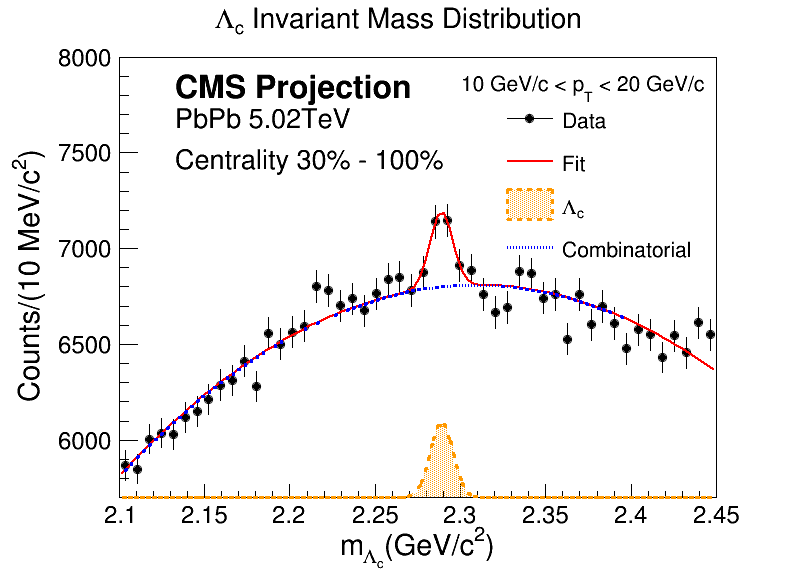
\includegraphics[width=85mm,scale=0.8]{LambdaC.png} \\}
\endminipage\hfill
\minipage{0.5\textwidth}
{\centering 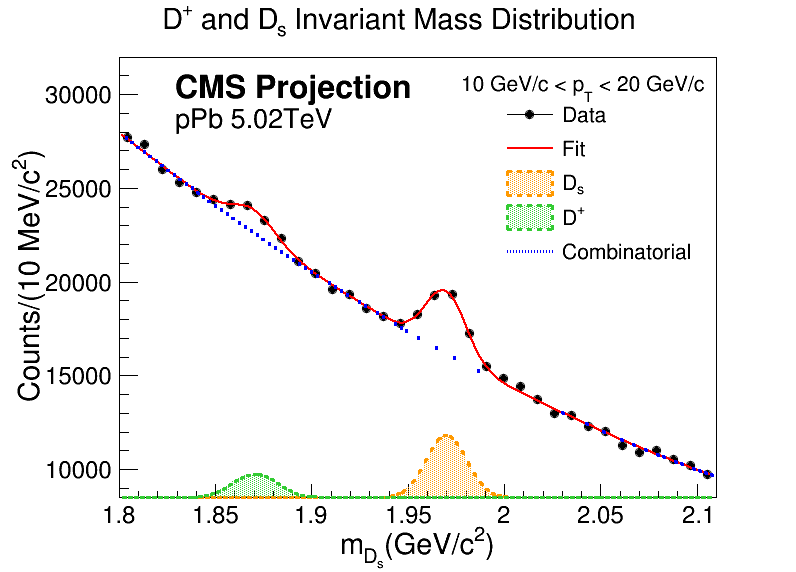
\includegraphics[width=85mm,scale=0.8]{Ds.png} \\}
\endminipage\hfill
 
\footnotesize \textbf{Fig. 1} The plots on the left is the invariant mass distribution of $\Lambda_C$ fitted with polynomial + Gaussian function and the right plot is the invariant mass distribution of $D_s$ fitted with polynomial + Gaussian function. 


\newpage \normalsize \textbf{Fitting Function and Parameters}

The fitting function is

\begin{equation}
f_{\Lambda_c}(x) = p_0 + p_1 x + p_2 x + p_3 e^{-\frac{(x-p_4)^2}{2 p_5^2}}
\end{equation}

\begin{equation}
f_{D_s}(x) = p_0 + p_1 x + p_2 x + p_3 e^{-\frac{(x-p_4)^2}{2 p_5^2}} + p_6 e^{-\frac{(x-p_7)^2}{2 p_8^2}}
\end{equation}

Here are the fitting parameters for the plots in figure 1. 
     
\vspace{1cm} \normalsize \begin{center}


\begin{tabular}{ |c|c|c| } 



\cline{1-3}
\multicolumn{3}{|c|}{\textbf{Fitting Parameter for $\Lambda_c$ and $D_s$} }\\
 \cline{1-3}
 Parameters    & $\Lambda_c$  & $D_s$ \\
            \cline{1-3}
$p_0$ & -1.15 $\times 10^5$ & 4.09 $\times 10^5$  \\
\hline 
$p_1$ & 1.05 $\times 10^5$ & -3.42 $\times 10^5$ \\
\hline
$p_2$ & -2.28 $\times 10^4$ & 7.23 $\times 10^4$ \\
\hline
$p_3$ & 3.94 $\times 10^2$ & 3.34 $\times 10^3$  \\
\hline
$p_4$ & 2.289 & 1.970 \\
\hline
$p_5$ &  6.52 $\times 10^{-3}$ & 1.04 $\times 10^{-2}$ \\
\hline
$p_6$ &   & 1.25 $\times 10^{3}$ \\
\hline
$p_7$ &  & 1.871 \\
\hline
$p_8$ &   & 1.14 $\times 10^{-2}$ \\
\hline

\end{tabular}
\end{center}







\end{document}
